\subsection{Full-Duplex Orchestrator}

\begin{figure}[ht]
\centering
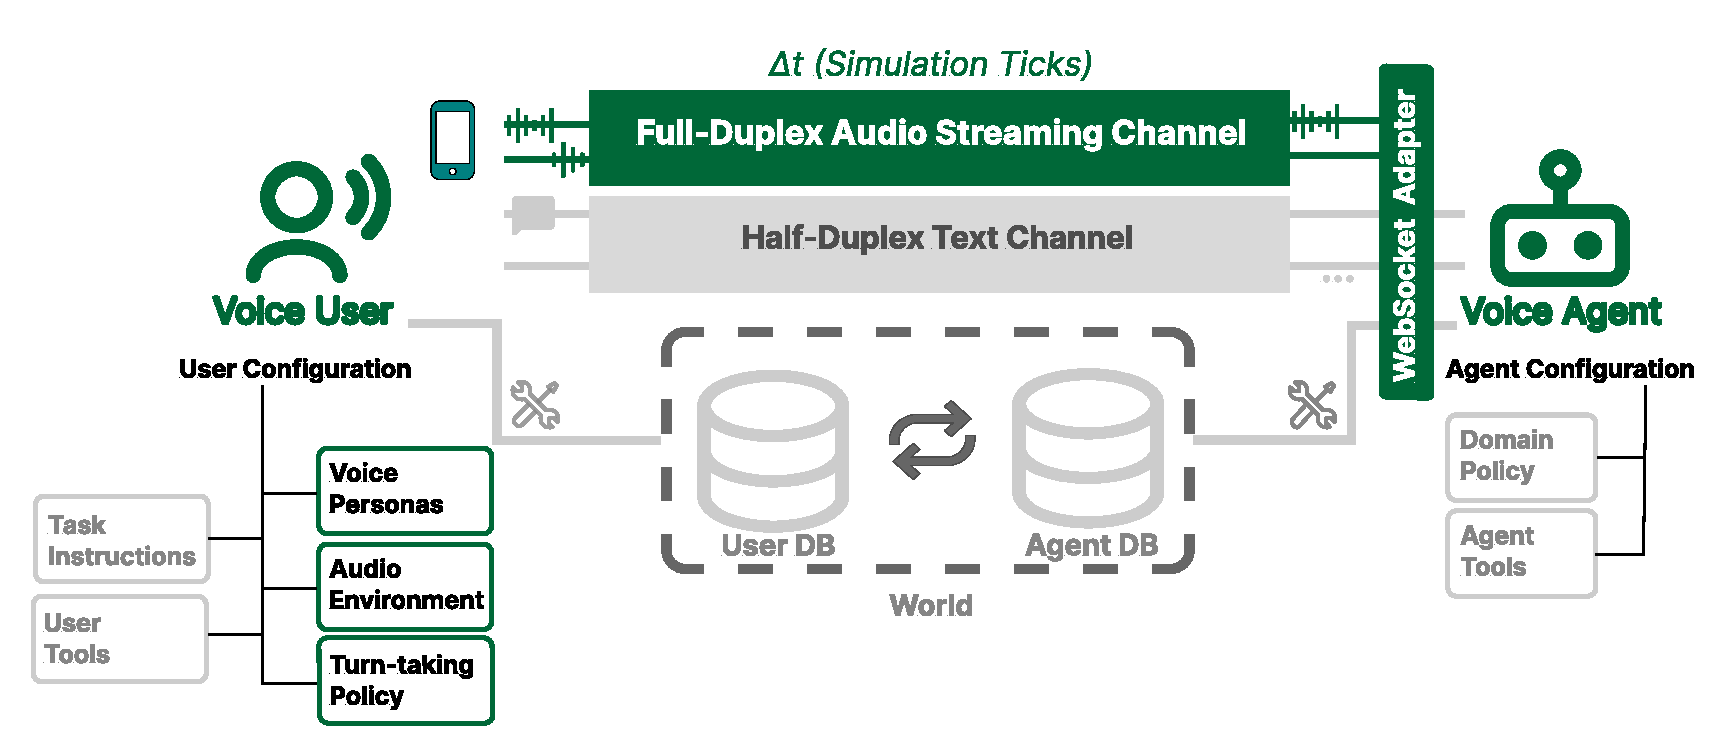
\includegraphics[width=\columnwidth]{figures/arch_diagram.pdf}
\caption{\tauvoice{} extends \tautwobench{} (gray) with voice-specific components (green): a voice user simulator with configurable personas, audio environment, and turn-taking policy; a full-duplex audio streaming channel discretized into simulation ticks; and a provider adapter for adding new voice APIs. Task infrastructure (instructions, tools, databases, domain policies) is inherited.}
\label{fig:architecture}
\end{figure}

The orchestrator coordinates the interaction loop between the voice user simulator and the agent API, managing audio exchange, turn-taking events, and evaluation logging. Voice agent APIs (OpenAI Realtime~\citep{openai_introducing_2025}, Gemini Live~\citep{vertex_ai_gemini_2025}, xAI Grok~\citep{xai_grok_voice_2025}) are designed for continuous real-time streaming with bidirectional audio flow and voice activity detection (VAD) for turn-taking. Crucially, these APIs index events on \textit{audio time} rather than wall-clock time---audio can be sent faster or slower than real-time and the API processes it according to audio timestamps.

This decoupling enables our tick-based orchestrator: by advancing simulation time independently of wall-clock time, we allow the user simulator to use the most capable LLM without real-time constraints, ensuring reliable instruction following and turn-taking decisions. This enables reproducibility and fine-grained control over the timing of all turn-taking actions.

\paragraph{Discrete Simulation Time.} We discretize the continuous audio stream into fixed-duration \textbf{ticks} ($\tau = 200$ms by default). Each tick, both parties exchange exactly $\tau$ ms of audio, enabling true full-duplex interaction where both can speak simultaneously. Since audio generation may not align with tick boundaries, both sides buffer; on interruption, the buffer is cleared, truncating the agent's in-progress response (formal details in Appendix~\ref{app:buffer-formalism}). The agent returns both audio and transcript text each tick, with text distributed proportionally to audio duration (Appendix~\ref{sec:proportional-text}); overlapping speech is linearized to sequential text for the user simulator LLM (Appendix~\ref{app:linearization}).

\paragraph{Controllability and Reproducibility.} Decoupling from real-time enables fine-grained control over all simulation parameters. Conversational dynamics are configurable: silence thresholds before responding, interruption check intervals, yield timing after overlap. The audio environment is fully parameterized: background noise SNR and drift, burst noise rate and intensity, telephony compression settings, and frame drop probability via a Gilbert-Elliott model. Voice personas specify accent, speaking style, and prosody. This enables systematic ablations isolating the impact of individual factors on task performance. Given a seed, all stochastic elements are deterministic for controlled comparison across agents; full reproducibility is limited only by LLM output variance.
